\documentclass[11pt, oneside]{article}

%
% Packages
%

\usepackage{geometry}
\geometry{letterpaper}
\usepackage[parfill]{parskip}      		% Activate to begin paragraphs with an empty line rather than an indent
\usepackage{graphicx}
\usepackage{booktabs}
\usepackage{topcapt}
\usepackage[labelfont =  {sf, bf}, textfont = sf, format = plain]{caption}
\usepackage{amssymb}
\usepackage{amsmath}
\usepackage{natbib}
\usepackage{color}
\usepackage{array}
\usepackage{gensymb}
\usepackage{setspace}
\newcommand{\stretchy}{1.5}
\usepackage{lineno}
\usepackage{textcomp}
\usepackage{cleveref}
\usepackage{subcaption}

% Make helvetica the default sans-serif font
% \renewcommand\sfdefault{phv}

% Package command for citing R packages
\newcommand{\pkg}[1]{{\fontseries{b}\selectfont #1}} 

% Setup


%
% Title and authors
%

\title{Grow with the flow: a latitudinal cline in physiology is associated with more variable precipitation in \textit{Erythranthe cardinalis}}
\author{Christopher D. Muir$^{1,*}$ and Amy L. Angert$^1$}
\date{}

%
% Start document
%

\usepackage{Sweave}
\begin{document}
\Sconcordance{concordance:ms.tex:ms.Rnw:%
1 77 1 1 47 13 1 1 0 53 1 1 10 56 1 1 113 39 1 1 18 4 1 1 46 1 1 1 47 3 %
1 1 16 3 1 1 12 11 1 1 50 1 5 9 1 1 222 255 1 1 17 51 1 1 14 51 1 1 14 %
49 1 1 15 56 1 1 11 89 1}

\maketitle

$^1$ Biodiversity Research Centre, University of British Columbia, Vancouver, BC, Canada \\
$^*$corresponding author: Chris Muir, cdmuir@biodiversity.ubc.ca \\

Running Head: Latitudinal cline and climate in \textit{Erythranthe} \\

Key words: local adaptation, cline, photosynthesis, growth rate, monkeyflower, \textit{Mimulus} \\

Data will be archived on Dryad upon publication. \\

%--------------------------------------------------
% Acknowledgements
%--------------------------------------------------

\section*{Acknowledgements}
Erin Warkman and Lisa Lin helped collect data. CDM was supported by a Biodiversity Postdoctoral Fellowship funded by the NSERC CREATE program. ALA was supported by an NSERC Discovery Grant and a grant from the National Science Foundation (DEB 0950171). Two anonymous referees provided constructive comments on earlier versions of this manuscript.

\clearpage

\setstretch{\stretchy}

\begin{center}
{\LARGE  \centering Grow with the flow: a latitudinal cline in physiology is associated with more variable precipitation in \textit{Erythranthe cardinalis}}
\end{center}

\section*{Abstract}

Local adaptation is commonly observed in nature: organisms perform well in their natal environment, but poorly outside it. Correlations between traits and latitude, or latitudinal clines, are among the most common pieces of evidence for local adaptation, but identifying the traits under selection and the selective agents is challenging. Here, we investigated a latitudinal cline in growth and photosynthesis across 16 populations of the perennial herb \textit{Erythranthe cardinalis} (Phrymaceae). Using machine learning methods, we identify interannual variation in precipitation as a likely selective agent: Southern populations from more variable environments had higher photosynthetic rates and grew faster. We hypothesize that selection may favor a more annualized life history -- grow now rather than save for next year -- in environments where severe droughts occur more often. Thus our study provides insight into how species may adapt if Mediterranean climates become more variable due to climate change.

\section*{Introduction}

% Toggle these commands to get version for doing word count
\linenumbers
% \pagenumbering{gobble}
% \raggedright

% Local adaptation and clines
Local adaptation has been documented within numerous species; populations generally have higher fitness in their native environment, but perform poorly outside it \citep{Schluter_2000, Leimu_Fischer_2008, Hereford_2009}. However, the prevalance of local adaptation remains difficult to assess because researchers rarely test for local adaptation unless there are obvious phenotypic or environmental differences (but see \citeauthor{Hereford_Winn_2008} \citeyear{Hereford_Winn_2008}). When local adaptation occurs, it frequently leads to clines in both phenotypes and allele frequencies when selection varies over environmental gradients \citep{Huxley_1938, Endler_1977, Barton_1999}. Phenotypic differences between populations along a cline often have a genetic basis and can be studied in a common garden \citep{Turesson_1922, Clausen_etal_1940, Hiesey_etal_1942}. Despite a long history of studying local adaptation and clines, it remains challenging to identify exactly which traits are under selection and which differ for nonadaptive reasons. In particular, the role that physiological differences play in local adaptation is poorly understood, despite the fact that physiology is frequently assumed to explain adaptation to the abiotic environment. A related problem is identifying which of the myriad and often covarying aspects of the environment causes spatially varying selective pressures. 

% Intrinsic versus plastic variation 
When populations are locally adapted, reaction norms for fitness will cross, such that local genotypes have higher fitness than foreign genotypes and rank orders change across environments \citep{Kawecki_Ebert_2004}. The traits that underlie local adaptation, however, need not mirror this pattern. Populations can have fixed genetic differences conferring trait values that are adaptive at home but neutral or maladaptive away. Alternatively, the ability to plastically respond to a particular environment or the magnitude of response to an environment could be adaptive. We distinguish between these patterns of adaptive trait differences by referring to `intrinsic' and `plastic' trait variation, respectively. Both intrinsic and plastic trait variation can be explained by genetic differences and both are involved in adaptation. For example, intrinsic differences in photoperiod responses \citep{Blackman_etal_2011} and developmental rate \citep{Stinchcombe_etal_2004} allow organisms to properly time their life history with the local environment. Conversely, sun and shade plants do not have intrinsically higher or lower rates of carbon assimilation, but rather, genotype-by-environment interactions cause sun plants to assimilate more under high light and shade plants under low light \citep{Givnish_1988}. In plants especially, we know little about the prevalence and adaptive significance of variation in fundamental physiological traits like photosynthesis and their impact on plant performance.

% Selective agents (trait-enviro assoc)
A basic approach to identify candidate traits underlying local adaptation is to find associations between traits and environments. Either intrinsic and/or plastic variation should vary clinally along environmental gradients. Indeed, clines in ecologically important traits are widespread in nature \citep{Endler_1977} and often adaptive, but in most cases the selective agent is unknown. For example, in \textit{Drosophila} numerous latitudinal clines exist for traits like thermal tolerance \citep{Hoffmann_etal_2002}, body size (\cite{Coyne_Beecham_1987} and references therein), and life history \citep{Schmidt_etal_2005}. Some \textit{Drosophila} clines have evolved multiple times (\cite{Oakeshott_etal_1982, Huey_etal_2000}, see also \cite{Bradshaw_Holzapfel_2001}) or shifted in response to climate change \citep{Umina_etal_2005}, evincing climatic adaptation. Similarly, plant species exhibit latitudinal clines in traits like flowering time \citep{Stinchcombe_etal_2004}, cyanogenesis \citep{Kooyers_Olsen_2012}, leaf morphology \citep{Hopkins_etal_2008, Stock_etal_2014}, and drought response \citep{Kooyers_etal_2015} that likely relate to climatic variation. 

Despite the fact that latitudinal clines have been studied for a long time, latitude \textit{per se} cannot be a selective agent. Latitude may be strongly correlated with one or two key climatic variables, such as temperature, precipitation, or growing degree-days. Latitude may also correlate with the strength of biotic interactions \citep{Schemske_etal_2009} or other nonclimatic aspects of the environment, though as we explain below, we do not yet have compelling data that these are important in our study system. Hence, we focus on whether latitude could be an effective proxy for an underlying climatic driver, in which case we would expect a yet stronger relationship between traits and the key climatic variable(s) driving selection. Alternatively, latitude may be more strongly related to traits than any single climatic variable for at least two reasons. First, latitude may be correlated with several climatic agents of selection that are individually weak, but add up to a strong latitudinal cline. Alternatively, gene flow among neighbouring populations could smooth out local climatic effects, since alleles will experience selection across populations linked by migration \citep{Slatkin_1978, Paul_etal_2011, Hadfield_2016}. We refer to this as the `climatic neighborhood'. For example, in mountainous regions average temperature at a given latitude varies widely, but in aggregate, a lower latitude set of populations will experience warmer climate than a higher latitude one. Thus, any particular low latitude population would be warm-adapted, even if it was located in a cooler (e.g. high elevation) site. Because many climatic factors vary latitudinally, and which climatic factors vary latitudinally changes over the earth's surface (e.g. coastal vs. continental), dissecting the evolution of latitudinal clines across many species will help identify generalities, such as whether thermal tolerance maxima or seasonal timing is more important \citep{Bradshaw_Holzapfel_2008}, and whether local or regional climate shapes selective pressures.

In this study, we investigated two major questions: 1) whether intrinsic or plastic physiological trait variation corresponds with latitude; and 2) what climatic factor(s) could plausibly be responsible for latitudinal clines. Within question 2, we tested three hypotheses outlined in the previous paragraph: latitudinal clines are explained by a single dominant climatic factor, multiple climatic factors, or the climatic neighborhood experienced by nearby population connected through gene flow. These hypotheses are not mutually exclusive since, for example, single or multiple factors in a climatic neighborhood may lead to latitudinal clines. We focused on climate because climate often determines and where species are found and also can exert strong selection on populations within species, though we acknowledge that other abiotic and biotic factors could also contribute to selection and the overall pattern of local adaptation. There is also a compelling need to know how populations are (or are not) locally adapted to climate so as to predict how they will respond to climate change \citep{Aitken_Whitlock_2013}. 

We examined these questions in \textit{Erythranthe cardinalis} (formerly \textit{Mimulus cardinalis} [\citeauthor{Nesom_2014} \citeyear{Nesom_2014}]) because linking physiological traits to potentially complex patterns of local adaptation requires integrating multiple lines of evidence from comparative, experimental, and genomic studies under both lab and field conditions. Many classic and contemporary studies of local adaptation use \textit{Mimulus sensu lato} species because of their natural history, easy propagation, and genetic/genomic resources \citep{Clausen_etal_1940, Hiesey_etal_1971, Bradshaw_Schemske_2003, Wu_etal_2008, Lowry_Willis_2010, Wright_etal_2013}. Yet, there is a deficiency of links between local adaptation and physiological mechanisms \citep{Angert_2006, Angert_etal_2008, Wu_etal_2010, Wright_etal_2013}. We measured genetic and genotype-by-environment variation in response to temperature and drought among 16 populations distributed over 10.7\textdegree of latitude. We found a latitudinal cline of intrinsic variation in photosynthesis and growth, but little evidence for variation in plasticity. Interannual variation in precipitation and temperature are associated with this axis of variation, suggesting that climatic variance rather than mean may be an important driver of local adaptation in \textit{E. cardinalis}. The climatic neighborhoods around populations explained trait variation better than local climate, indicating that latitudinal clines may be common because latitude integrates effects of selection on populations connected through gene flow. We place these findings in the context of life history theory and consider future directions in the Discussion. 

\section*{Material and Methods}


\subsection*{Population Selection}

\textit{E. cardinalis} is a perennial forb native to the Western US (California and Oregon). It is predomintantly outcrossing, self-compatible, and pollinated primarily by hummingbirds. We used 16 populations from throughout the range of \textit{E. cardinalis} (Table~\ref{table:Table_FocalPops}). These populations were intentionally chosen to span much of the climatic range of the species based on all known occurrences (see below). Seeds were collected in the field from mature, undehisced fruit left open for 2-4 weeks to dry, then stored at room temperature. We used seeds from 154 families, 4--12 (mean = 9.6, median = 12) families per population.


%%%%%%%%%%%%%%%%%%%%%%%%%%%%%%%%%%%%%%%%%%%%%%%%%%%%%%%%%%%%%%%%%%%%%%%%%%%%%%%%
% Table of focal population
%%%%%%%%%%%%%%%%%%%%%%%%%%%%%%%%%%%%%%%%%%%%%%%%%%%%%%%%%%%%%%%%%%%%%%%%%%%%%%%%

\begin{table}[ht]
   \centering
   \topcaption[Focal Populations]{Latitude, longitude, and elevation (mas = meters above seal level) of 16 focal populations used in this study.}
   \begin{tabular}{@{} llll @{}}
      \toprule
  Name  & Latitude  & Longtiude  & Elevation (mas) \\
      \midrule
	Hauser Creek & 32.657	& 
    -116.532	& 799   \\
	Cottonwood Creek	& 32.609 & 
    -116.7	& 267   \\
	Sweetwater River	& 32.9 & 
    -116.585	& 1180   \\
	Grade Road Palomar & 33.314 &
    -116.871	& 1577   \\
	Whitewater Canyon & 33.994 & 
    -116.665	& 705   \\
	Mill Creek	& 34.077 & 
    -116.873	& 2050   \\
	West Fork Mojave River	& 34.284 & 
    -117.378	& 1120   \\
	North Fork Middle Tule River	& 36.201 & 
    -118.651	& 1314   \\
	Paradise Creek	& 36.518 & 
    -118.759	& 926   \\
	Redwood Creek	& 36.691 & 
    -118.91	& 1727   \\
	Wawona  & 37.541 & 
    -119.649	& 1224   \\
	Rainbow Creek	& 37.819 & 
    -120.007	& 876   \\
	Middle Yuba River	& 39.397 & 
    -121.082	& 455   \\
	Little Jamison Creek	& 39.743 & 
    -120.704	& 1603   \\
	Deep Creek	& 41.668 & 
    -123.11	& 707   \\
	Rock Creek	& 43.374 & 
    -122.957	& 326   \\
	\bottomrule
	\end{tabular}
	\label{table:Table_FocalPops}
\end{table}

\subsection*{Plant propagation}

On 14 April, 2014, 3-5 seeds per family were sown directly on sand (Quikrete Play Sand, Georgia, USA) watered to field capacity in RLC4 Ray Leach cone-tainers placed in RL98 98-well trays (Stuewe \& Sons, Inc., Oregon, USA). We used pure sand because \textit{E. cardinalis} typically grows in sandy, riparian soils (A. Angert, pers. obs.). Two jumbo-sized cotton balls at the bottom of cone-tainers prevented sand from washing out. Cone-tainers sat in medium-sized flow trays (FLOWTMD, Stuewe \& Sons, Inc., Oregon, USA) to continuously bottom-water plants during germination in greenhouses at the University British Columbia campus in Vancouver, Canada (49\degree 15' N, 123\degree 15' W). Misters thoroughly wetted the top of the sand every two hours during the day. Most seeds germinated between 1 and 2 weeks, but we allowed 3 weeks before transferring seedlings to growth chambers. We recorded germination daily between one to two weeks after sowing, and every 2-3 days thereafter. On 5 May (21 days after sowing), we transferred seedlings to one of two growth chambers (Model E-15 Conviron, Manitoba, Canada). We thinned seedlings to one plant per cone-tainer, leaving the center-most plant. 702 of 768 (91.4\%) had plants that could be used in the experiment. We allowed one week at constant, non stressful conditions (day: 20\celsius, night: 16\celsius) for plants to acclimate to growth chambers before starting treatments. The initial size of seedlings, measured as the length of the first true leaves, did not differ between populations, families, or treatments (Table~\ref{table:TableS_InitialSize}).
    
\subsection*{Temperature and drought treatments}

We imposed four treatments, a fully-factorial cross of two temperature levels and two watering levels. The temperature levels closely simulated an average growing season at the thermal extremes of the species range, which we designate as Hot and Cool treatments. Watering levels contrasted a perennial and seasonal stream, which we refer to as Well-watered and Drought treatments. A detailed description of treatments is provided in the Supplemental Materials and Methods and summarized in Fig~\ref{fig:Fig_ExptlDes}. Because growth chambers cannot be subdivided, one chamber was assigned to the Hot treatment level and another to the Cool treatment level. Within each chamber, there were two Well-watered blocks and two Drought blocks. The photosynthetically active radiation in both chambers was approximately 400 $\mu$mol quanta m$^{-2}$ s$^{-1}$. The growth chambers did not control humidity, but because of watering and high plant transpiration rates, the relative humidity was quite high in both temperature levels (data not shown). Lower humidity would have made the drought more severe, but low soil moisture is stressful in and of itself. The total number of plants in each treatment was: $n_{\text{cool,dry}} = 169$; $n_{\text{cool,ww}} = 174$; $n_{\text{hot,dry}} = 176$; $n_{\text{hot,ww}} = 183$. Each population had 8--12 individuals per treatment level (mean = 11, median = 11).


%%%%%%%%%%%%%%%%%%%%%%%%%%%%%%%%%%%%%%%%%%%%%%%%%%%%%%%%%%%%%%%%%%%%%%%%%%%%%%%%
% Figure summarizing experimental design
%%%%%%%%%%%%%%%%%%%%%%%%%%%%%%%%%%%%%%%%%%%%%%%%%%%%%%%%%%%%%%%%%%%%%%%%%%%%%%%%

\begin{figure}[h!]
	\centerline{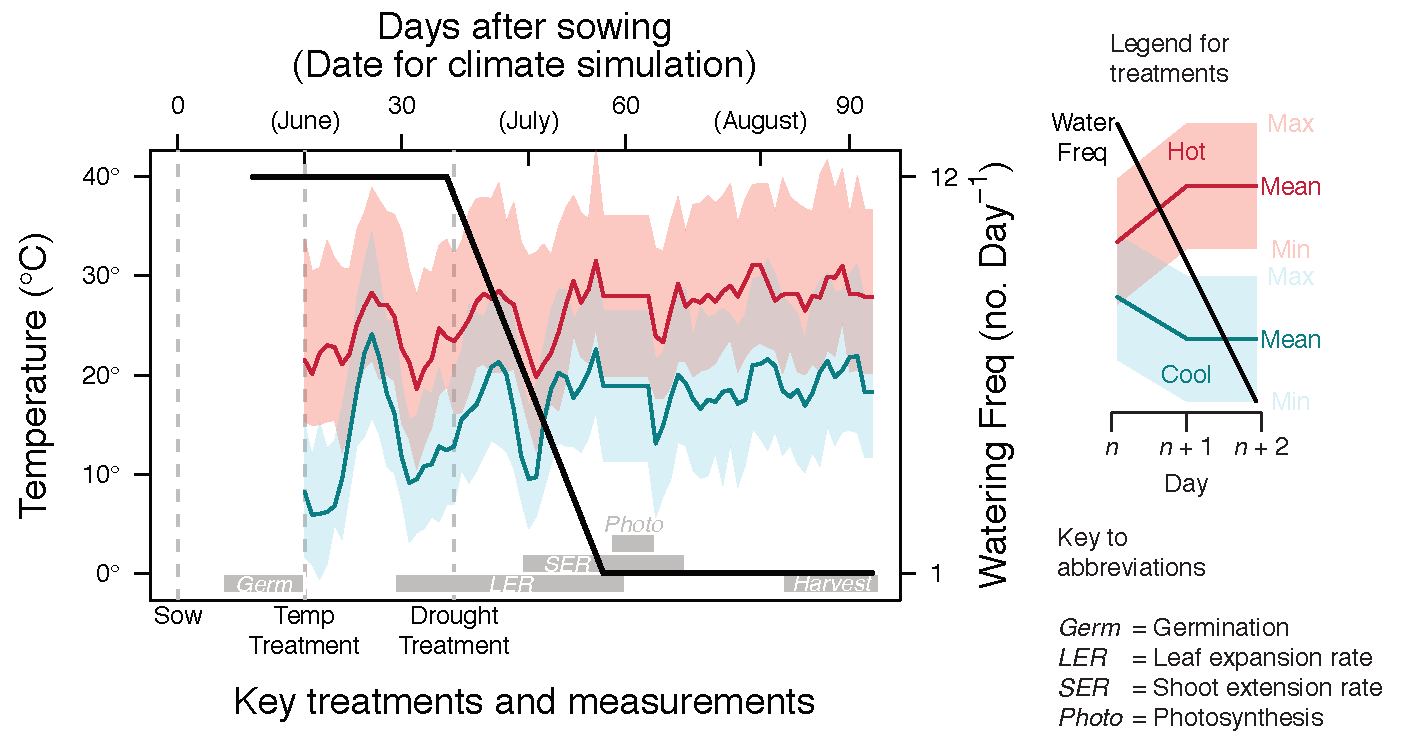
\includegraphics[width=1\textwidth]{Figures/Figure_ExptlDes.pdf}}
	\usefont{T1}{phv}{m}{n}
	\fontsize{10}{12}
	\selectfont
	\caption[Experimental Design]{Overview of experimental treatments and timing of key trait measurements. All plants germinated within 21 days of sowing. At that time, we began temperature treatments (left axis), simulating a typical June-August weather pattern at Hot (red) and Cool (blue) sites. The bold lines track the average daily temperatures. Within each day, there was a maximum daytime temperature (top of translucent polygons) and minimum nighttime temperature (bottom of translucent polygons). The drought treatment commenced later by ramping down the frequency of bottom-watering episodes (dashed black line; right axis), while watering frequency was maintained in the control treatment (solid black line). Grey boxes on the bottom of the plot outline the period of key measurements described in the Material and Methods.}
	\label{fig:Fig_ExptlDes}
\end{figure}

\subsection*{Trait measurements}

We measured five traits in response to temperature and watering treatments (Table~\ref{table:Table_traits}).

%%%%%%%%%%%%%%%%%%%%%%%%%%%%%%%%%%%%%%%%%%%%%%%%%%%%%%%%%%%%%%%%%%%%%%%%%%%%%%%%
% Table of key traits
%%%%%%%%%%%%%%%%%%%%%%%%%%%%%%%%%%%%%%%%%%%%%%%%%%%%%%%%%%%%%%%%%%%%%%%%%%%%%%%%

\begin{table}[ht]
   \centering
   \topcaption{Key traits measured in this study.}
   \begin{tabular}{@{} ll @{}}
      \toprule
  Trait & Units \\
      \midrule
  Days to germination  & day \\
  Leaf expansion rate  &  mm day$^{-1}$  \\
  Stem elongation rate  &  cm day$^{-1}$  \\
  Photosynthetic rate &  $\mu$mol CO$_2$ m$^{-2}$ s$^{-1}$\\
  Mortality & probability of death  \\
	    \bottomrule
   \end{tabular}
   \label{table:Table_traits}
\end{table}

\paragraph{Days to germination} We tested for population variation in germination rate, measured as Days to Germination, using a lognormal survival model fit using the survreg function in the R package \pkg{survival} version 2.38 \citep{Therneau_2015}. We treated Population as a fixed effect and Family as random effect using a $\Gamma$ frailty function. Statistical significance of the Population effect was determined using analysis of deviance. Note that, unlike other traits discussed below, we did not include Block, Treatment, or Population $\times$ Treatment interactions because during germination plants had not been placed into blocks and treatments had not yet been applied.


\paragraph{Growth rate: leaf expansion and stem elongation}

We measured growth rate during two phases: leaf expansion and stem elongation. Growth measurements were taken during the early vegetative stage. We censused leaf length twice per week shortly after the emergence of true leaves from 12 May -- 12 June (28--59 days after sowing), resulting in 10 measurements. We ceased measuring leaf length once it appeared to asymptote and growth shifted to stem elongation. We also censused plant height on 7 occasions (twice per week) between 29 May and 20 June (45 to 67 days after sowing) until plants began to initiate floral buds. Thus all growth measurements occured during the vegetative, prereproductive phase. Both leaf expansion and stem elongation were modelled separately as second-order polynomials. We used empirical Bayes' estimates of growth for each individual plant from linear mixed-effects models fit with the R package \pkg{lme4} version 1.1-12 \citep{Bates_etal_2015}.




\paragraph{Photosynthesis}
During the week of 10 to 16 June (57 to 63 days after sowing), we measured daytime photosynthetic rate on a subset of 329 plants evenly spread between treatments and families within populations. The youngest, fully-expanded leaf acclimated for 3 minutes to reach steady state in a 6-cm$^2$ chamber of a LI-COR 6400XT Portable Photosynthesis System (LI-COR Biosciences, Lincoln, Nebraska). We made all measurements at ambient light (400 $\mu$mol m$^{-2}$ s$^{-1}$ of photosynthetically active radiation), atmospheric CO$_2$ (400 ppm), temperature, and moderate relative humidity. During this period, we suspended normal day-to-day temperature fluctuations and set daytime temperatures to the average for that period (Cool: 26.5$\degree$; Hot: 36.1$\degree$) so that all plants within a temperature level could be measured under the same conditions.


\paragraph{Mortality}
We assayed mortality during twice-weekly growth measurements. We analyzed the probability of surviving until the end of the experiment as a function of population, treatment, and their interactions using a Generalized Linear Mixed Model (GLMM) assuming binomially distributed errors. We included Family and Block as random effects. We assessed significance of fixed effects using Type-II Analysis of Deviance with Wald $\chi ^2$ tests in the R package \pkg{car} \citep{Fox_Weisberg_2011}. 


\subsection*{Intrinsic variation and plasticity}

For all traits (Table~\ref{table:Table_traits}) except germination (see above), we tested for Population, Treatment (Temperature, Water, and Temperature $\times$ Water), and Population $\times$ Treatment interactions (Population $\times$ Temperature, Population $\times$ Water, and Population $\times$ Temperature $\times$ Water). We interpreted significant Population effects to indicate intrinsic variation and Population $\times$ Treatment interactions to indicate variation in plasticity. As mentioned above, we used survival and GLMM models for germination rate and mortality, respectively. For all other traits, we used mixed model ANOVAs with Family and Block included as random factors. We fit models using restricted maximum likelihood in lmer, a function in the R package \pkg{lme4} \citep{Bates_etal_2015}. We determined significant fixed effect terms using a step-wise backward elimination procedure implemented with the step function in the R package \pkg{lmerTest} version 2.0-32 \citep{Kuznetsova_etal_2016}. This package uses Satterthwaite's approximation to calculate denominator degrees of freedom for $F$-tests. We also included days to germination as a covariate in growth analyses. To ensure that Population and Treatment effects were specific to a particular growth phase, we included germination day as a covariate in leaf expansion and stem elongation analyses.

\subsection*{Principal components of germination, growth, and photosynthesis}
For each single-trait model above, we extracted the Population coefficient (factoring out Treatment and other effects). The multivariate distribution of these coefficients was then summarized using principal components analysis. The first principal component of these traits (TraitPC1) loaded positively with germination, growth, and photostynthetic rate, therefore we define this as a phenotypic axis delineating fast to slow growth.



\subsection*{Identifying putative selective agents}

Latitudinal clines are common, but it is often difficult to ascribe this variation to a particular selective agent. To reiterate, we tested three non-mutually exclusive hypotheses about how such latitudinal clines emerge: 1) one or two climatic variables explain latitudinal trait variation; 2) latitude is a proxy for multiple climatic factors that together shape trait variation; and 3) latitude integrates selection in a broader climatic neighborhood. We found that a population's position along TraitPC1 correlated strongly with the latitude of origin (see Results) and next used Random Forest regression \citep{Liaw_Wiener_2002} to identify putative climatic factors underlying trait-latitude associations in \textit{E. cardinalis}. We reasoned that if we identified a single climatic factor that explained more trait variation than latitude, then this would suggest that factor is a key selective agent underlying the latitudinal cline (Hypothesis 1). On the other hand, if multiple climatic factors together are necessary to explain trait variation, then this would suggest that many climatic factors together have imposed selection for the latitudinal cline (Hypothesis 2). We hereafter refer to factors identified in this analysis as `Climate-TraitPC1' variables. To test Hypothesis 3 about climatic neighborhoods driving selection, we directly competed local with neighborhood climate. We used the immediate collection location for local climate. For climate neighborhoods, we sampled climate at 1000 random points (at 90-m resolution) within a 62-km radius buffer around the collection and took the average. We chose this buffer radius based on population genetic structure, as inferred from $\approx$25,000 restriction-site associated SNPs among 49 populations from across the range \citep{Paul_etal_2016}. Spatial autocorrelation in allele frequencies persists for 62 km. However radii of 10 km$^2$ and 100 km$^2$ resulted in similar outcomes (data not shown). Since \textit{E. cardinalis} is found exclusively in riparian areas, we only selected points along streams using the National Hydrogeoraphy Dataset \citep{NHD}. Climatic means and variances (see below) were weighted by their climatic suitability as determined using a multimodel ensemble average of ecological niche models \citep{Angert_ENM}. In addition to competing local and neighborhood climate, we compared the univariate correlation between local and neighborhood climate with TraitPC1 and Latitude using paired $t$-tests. We adjusted degrees of freedom to account for the fact that many climatic factors are highly correlated and not independent. Specifically, we calculated the effective number of independent climatic factors ($M_\text{eff}$) using the formula $M_\text{eff} = 1 + (M - 1) (1 - \text{Var}(\lambda) / M)$ \citep{Chevrud_2001}, where $M$ is the original number of climatic factors and $\lambda$ are the eigenvalues of the correlation matrix of all climatic factors. 

To help eliminate potentially spurious correlations between TraitPC1 and climate, we tested for overlap between climatic variables that best predict latitude of all \textit{E. cardinalis} occurrence records (see detail below), not just the 16 focal populations. We refer to these climatic factors as `Climate-Latitude' variables. The logic is that climatic factors associated with both TraitPC1 and latitude for all populations are more likely to be important selective agents than climatic factors that happen to correlate with TraitPC1 but do not covary with latitude throughout the \textit{E. cardinalis} range. Therefore, we did not consider Climate-TraitPC1 variables to be candidate selective agents unless the same or very similar variable was found in the Climate-Latitude analysis. However, we do interpret potential selective agents identified in Climate-Latiude analyses alone, because the goal was to explain the latitudinal clines in traits, not all aspects of climate that vary with latitude.

We selected Climate-Latitude and Climate-TraitPC1 variables independently using Variable Selection Using Random Forest (VSURF) algorithm in the R package \pkg{VSURF} version 1.0.3 \citep{Genuer_etal_2016}. Random Forest regression is useful for cases like ours when the number of potential predictors is similar to or greater than the number of observations (`high $p$, low $n$' problem). VSURF is a multistip algorithm that progressively retains or eliminates variables based on their importance over regression trees in the forest. Variable importance is defined as the average amount a climate variable reduces mean-squared error in the predicted response (TraitPC1 or Latitude), compared to a randomly permuted dataset, across all trees in the random forest (see \citeauthor{Genuer_etal_2015} [\citeyear{Genuer_etal_2015}] for further detail). Hence, VSURF automatically eliminates unimportant and redundant variables based on the data without having to arbitrarily choose among colinear climate variables before the analysis. We kept only variables selected for prediction, the most stringent criterion. A visual overview of how we selected climatic variables is depicted in Fig~\ref{fig:Fig_VarSelect}. 

